
\documentclass[a4paper,10pt,fleqn, twocolumn]{IEEETran}
\usepackage{amsfonts}
\usepackage{amsthm}
\usepackage{graphicx}
\usepackage{fancyhdr}



\setlength{\parindent}{3em} \setlength{\oddsidemargin}{0in}
\setlength{\textwidth}{6.5in} % sets 1in left and right margins
\setlength{\topmargin}{0.20in} % change to 0.2in for regular latex
%\setlength{\headheight}{0in}
%\setlength{\footheight}{0.5in}
\setlength{\footskip}{0.5in}
\setlength{\textheight}{9.0in} %sets 1in top and bottom margins
\renewcommand{\baselinestretch}{1} %set to 1.5 for double spacing.



\newcommand{\br}{{\mathbf r}}
\newcommand{\bA}{{\mathbf A}}
\newcommand{\ba}{{\bf a}}
\newcommand{\bb}{{\bf b}}
\newcommand{\bc}{{\bf c}}
\newcommand{\bC}{{\bf C}}
\newcommand{\bg}{{\bf g}}
\newcommand{\bG}{{\bf G}}
\newcommand{\bd}{{\bf d}}
\newcommand{\be}{{\bf e}}
\newcommand{\bs}{{\bf s}}
\newcommand{\bm}{{\bf m}}
\newcommand{\bn}{{\bf n}}
\newcommand{\bu}{{\bf u}}
\newcommand{\bv}{{\bf v}}
\newcommand{\bw}{{\bf w}}
\newcommand{\bx}{{\bf x}}
\newcommand{\by}{{\bf y}}
\newcommand{\bbf}{{\bf f}}
\newcommand{\bE}{{\bf E}}
\newcommand{\bF}{{\bf F}}
\newcommand{\bL}{{\bf L}}
\newcommand{\bM}{{\bf M}}
\newcommand{\bN}{{\bf N}}
\newcommand{\bS}{{\bf S}}
\newcommand{\bT}{{\bf T}}
\newcommand{\bD}{{\bf D}}
\newcommand{\bX}{{\bf X}}
\newcommand{\bP}{{\bf P}}
\newcommand{\bQ}{{\bf Q}}
\newcommand{\bI}{{\bf I}}
\newcommand{\bR}{{\bf R}}
\newcommand{\bU}{{\bf U}}
\newcommand{\bV}{{\bf V}}
\newcommand{\bW}{{\bf W}}
\newcommand{\bJ}{{\bf J}}
\newcommand{\bB}{{\bf B}}
\newcommand{\bzero}{{\bf 0}}
\newcommand{\bgamma}{{\mbox {\boldmath $\gamma$}}}
\newcommand{\btheta}{{\mbox {\boldmath $\theta$}}}
\newcommand{\bLambda}{{\mbox {\boldmath $\Lambda$}}}
\newcommand{\bPsi}{{\mbox {\boldmath $\Psi$}}}
\newcommand{\bPhi}{{\mbox {\boldmath $\Phi$}}}
\newcommand{\bcA}{{\mbox {\boldmath ${\cal A}$}}}
\newcommand{\bcB}{{\mbox {\boldmath ${\cal B}$}}}
\newcommand{\bcC}{{\mbox {\boldmath ${\cal C}$}}}
\newcommand{\bcD}{{\mbox {\boldmath ${\cal D}$}}}
\newcommand{\bcF}{{\mbox {\boldmath ${\cal F}$}}}
\newcommand{\bcN}{{\mbox {\boldmath ${\cal N}$}}}
\newcommand{\bcS}{{\mbox {\boldmath ${\cal S}$}}}
\newcommand{\bcH}{{\mbox {\boldmath ${\cal H}$}}}
\newcommand{\bcI}{{\mbox {\boldmath ${\cal I}$}}}
\newcommand{\bcR}{{\mbox {\boldmath ${\cal R}$}}}

\title{Blind Adaptive Multiuser Detection}
\author{Shu Wang, Sang G. Kim, Li-Hsiang Sun, Hobin Kim,\\
   Suk W. Lee, S. R. Subramanya, Ki Y. Kim and Byung K. Yi\\ LGE Mobile Research (LGEMR), San Diego, CA 92131}
\date{}
\begin{document}
\maketitle
\begin{abstract}\small
In this paper, we propose a new blind multiuser detection
framework and several blind detectors for solving the near-far
problem in synchronous CDMA. Compared with existing blind
multiuser detectors, the proposed detectors require a minimum
number of previously received signals, which is equal to the
number of unknown interfering users, and no subspace separation or
channel/sequence estimation operation. Hence their computation
complexity and detection delay are much reduced. To achieve this,
a blind multiuser detection model is used with least squares (LS)
estimation, best least unbiased (BLU) estimation and minimum
mean-square error (MMSE) estimation criteria instead of the
popular conventional multiuser model and/or subspace-based
parametric model. A recursively adaptive procedure is further
developed for decreasing the complexity. All these can be easily
extended for asynchronous CDMA. Theoretical analysis and computer
simulations are provided to demonstrate the performance of the
proposed schemes.
\end{abstract}
\section{Introduction}
Multiuser detection strategy is a method for mitigating multiple
access interference (MAI) effects and solving the near-far problem
with exploiting interference structure~\cite{Verd98}. Recent
research has been devoted to blind multiuser detection and
subspace-based signature waveform estimation schemes for blind
reducing required computation complexity and prior
knowledge~\cite{Madh94,Honi95,Torl97,Wang98,Wang99,Zhang02}. Blind
multiuser detectors can achieve good performance with only the
knowledge of the timing and signature waveform of desired user(s).
This assumption is also much closer to practical applications.
There are two popular approaches for designing blind multiuser
detectors. One is to use the conventional multiuser signal
model~\cite{Verd98}, where received signals and multiuser
receivers are taken as linear combinations of actual spreading
sequences and noise, and statistical signal estimation techniques
for blind multiuser detection, e.g., the blind multiuser receiver
design using Wiener filters~\cite{Madh94,Honi95} or Kalman
filters~\cite{Zhang02} techniques. The other approach is based on
parametric signal modelling and signal spectrum estimation, where
received signals and multiuser receivers are taken as a linear
combination of desired users' spreading sequences and the
signal/noise subspace bases. Many subspace-based schemes are
examples of this approach, which essentially is an approach for
blindly reconstructing existing conventional multiuser detectors
using subspace concept~\cite{Wang98,Wang99}. One of the
difficulties in implementing the above approaches is that the
signal bases employed for designing blind multiuser receivers are
mostly unknown beforehand and it is nontrivial to accurately
estimate them. Therefore the required computation resources are
known to be very high for many practical applications, especially
when wireless channels or active users experience fast dynamic
change.

In order to solve the near-far problem with minimum prior
knowledge and computation complexity, we propose a new blind
multiuser framework based on a blind multiuser signal model in
this paper. This blind signal model is different from the
traditional linear prediction model~\cite{Haykin96}~\footnote{The
discussion of the relationship between linear prediction and the
proposed framework is omitted because of the paper length
limitation.} and the widely-discussed conventional signal model
and subspace-based parametric signal model. In the proposed model,
each received signal can be taken as a linear combination of
desired users' spreading sequences, several previously received
signals and/or noise. Based on this new blind multiuser signal
model and detection framework, several blind multiuser detectors
are developed using best linear unbasied and minimum mean squared
error estimation criteria in addition to the least-squares-based
schemes in~\cite{Wang03d,Wang03e}. The proposed algorithms are
simple and direct only using the signatures and timing of desired
users. There is no converging, estimation or subspace separation
procedure employed by many other blind
detectors~\cite{Madh94,Honi95,Wang98,Wang99}. Compared with
existing blind detection schemes, they require a minimum number of
previously received signals. Hence the computation complexity and
detection delay can be much reduced. A recursively adaptive
implementation is provided to further lessen the required
computation complexity. The near-far performance and the trade-off
between the complexity and performance are also discussed.
Computer simulations are finally presented to demonstrate the
performance of these blind detectors.
\section{System Model And Problem Description}
We consider forward-link transmissions in a single-cell DS/CDMA
system. There are $K$ active users over the multipath channel with
$P$ strong paths~\footnote{Strong paths are those to be explicitly
combined by RAKE receiver.} and the channel is an additive white
Gaussian noise (AWGN) channel. The baseband representation of the
received signal due to user $k$ is given by
\begin{equation}
\begin{array}{rcl}
r_k(t)&=&\sum\limits_{p=1}^{P}\alpha_{pk}A_k[n]
b_k[n]c_k(t-nT-\tau_p)
\end{array}
\end{equation}
\noindent where $\alpha_{pk}$ is the $p$th path loss of user $k$'s
signal, $b_k{[n]}$ is the $n$th bit sent by user $k$. We assume
that the $\left\{b_k{[n]}\right\}$ are independent and identically
distributed random variables with $E\left\{b_k{[i]}\right\}=0$ and
$E\left\{|b_k{[i]}|^2\right\}=1$. The parameters $c_k(t)$ denote
the normalized spreading signal waveform of user $k$ during the
interval $[0,\ T]$, $0\leq\tau_1\leq\tau_2\leq\ldots\leq\tau_P$,
denotes $P$ different transmission delays from the base station to
user $k$ and $A_k[n]$ is the received signal amplitude for user
$k$ at time $t=n$, which depends on the possible channel
statistics. The total baseband signal received by user $k$ is
\begin{equation}
\begin{array}{rcl}
\tilde{r}(t)&=&\sum\limits_{k=1}^{K}r_k(t)
\end{array}
\end{equation}
The received signal $\tilde{r}(t)$ is passed through the
corresponding chip matched filter (CMF), $\phi(t)$, and RAKE
combiner. The combined output $r(t)$ is~\footnote{Without loss of
the generality, we drop the time index $n$ in the following
discussion.}
\begin{equation}\hspace{-0.0in}
\begin{array}{rcl}
r(t)&=&A_k b_k c_k(t-nT-\tau_1)\otimes \phi(t-\tau_1)+ \\
&&\hspace{0.0in} m_{\rm ISI}(t) + m_{\rm MAI}(t) + n(t)
\end{array}\label{r_t}
\end{equation}
\noindent where
\begin{equation} \hspace{-0.05in}
\begin{array}{rcl}
 m_{\rm ISI}(t)&=&\\
 &&\hspace{-0.83in}\sum\limits^{P}_{p\neq
q}\beta_{qk} \alpha_{pk}A_kb_kc_k(t-nT+\tau_{q1}-\tau_1)\otimes
\phi(t-\tau_1)
\end{array}
\end{equation}
\noindent is the intersymbol interference (ISI) to user $k$,
\begin{equation} \hspace{-0.17in}
\begin{array}{rcl}
m_{\rm MAI}(t)&=&\sum\limits_{i\neq
 k}^{K}A_ib_ic_i(t-nT-\tau_1)\otimes\phi(t-\tau_1)+\\
 &&\hspace{-0.75in}\sum\limits_{i\neq
 k}^{K}\sum\limits^{P}_{p\neq
q}\beta_{qk}
\alpha_{pi}A_ib_ic_i(t-nT+\tau_{q1}-\tau_p)\otimes\phi(t-\tau_1)
\end{array}
\end{equation}
\noindent is the MAI to user $k$, $\beta_{qk}$ is the weight of
the $q$th RAKE finger with
$\sum\limits_{q=1}^{P}\beta_{qk}\alpha_{qk}=1$ and $\tau_{q1} =
\tau_{q}-\tau_1$ is the propagation delay difference between the
$1$st path and $p$th path. $\otimes$ denotes the convolutional
product. $n(t)$ is AWGN with variance $\sigma^2$. The user $k$'s
RAKE output can be sampled at $f_s=1/T_s$ and straightforwardly
expressed by
\begin{equation}\hspace{-0.1in}
\begin{array}{rcl}
\br&=&\left[
\matrix{r(nT+T_s+\tau_1)&\ldots&r(nT+LT_s+\tau_1)}\right]^{\rm
T}\\
 &=&\sum\limits_{k=1}^{K} A_k b_k \bs_k + \bn \\
 &=&\bS \bA \bb + \bn
\end{array}\label{r_sync}
\end{equation}
\noindent where $\bS=[\bs_1\ \bs_2\ \ldots\ \bs_K]$ is the
received spreading sequence matrix combined with both ISI and MAI
information, and $L=T/T_s$ is the number of samples per symbol,
which should not be less than the spreading gain $L_c$.

Because of $m_{\rm MAI}(t)$ existing in the received signal
$r(t)$, the performance of conventional matched filter receiver
suffers from the so-called near-far problem~\cite{Verd98}.
Multiuser detection is the receiver technique for solving this
problem and most multiuser detectors are developed using the
conventional system model like (\ref{r_sync}). These are well
documented in~\cite{Verd98}. One of the difficulties in developing
blind multiuser detectors using (\ref{r_sync}) is that the $\bS$
is hard to be known beforehand. And it normally takes much effort
to determine it later. The similar situation arises in developing
blind detectors using the parametric subspace signal model
proposed in~\cite{Wang98}.
\section{Blind Multiuser Detection Framework\label{BMUD_model}}
\begin{figure} \center{
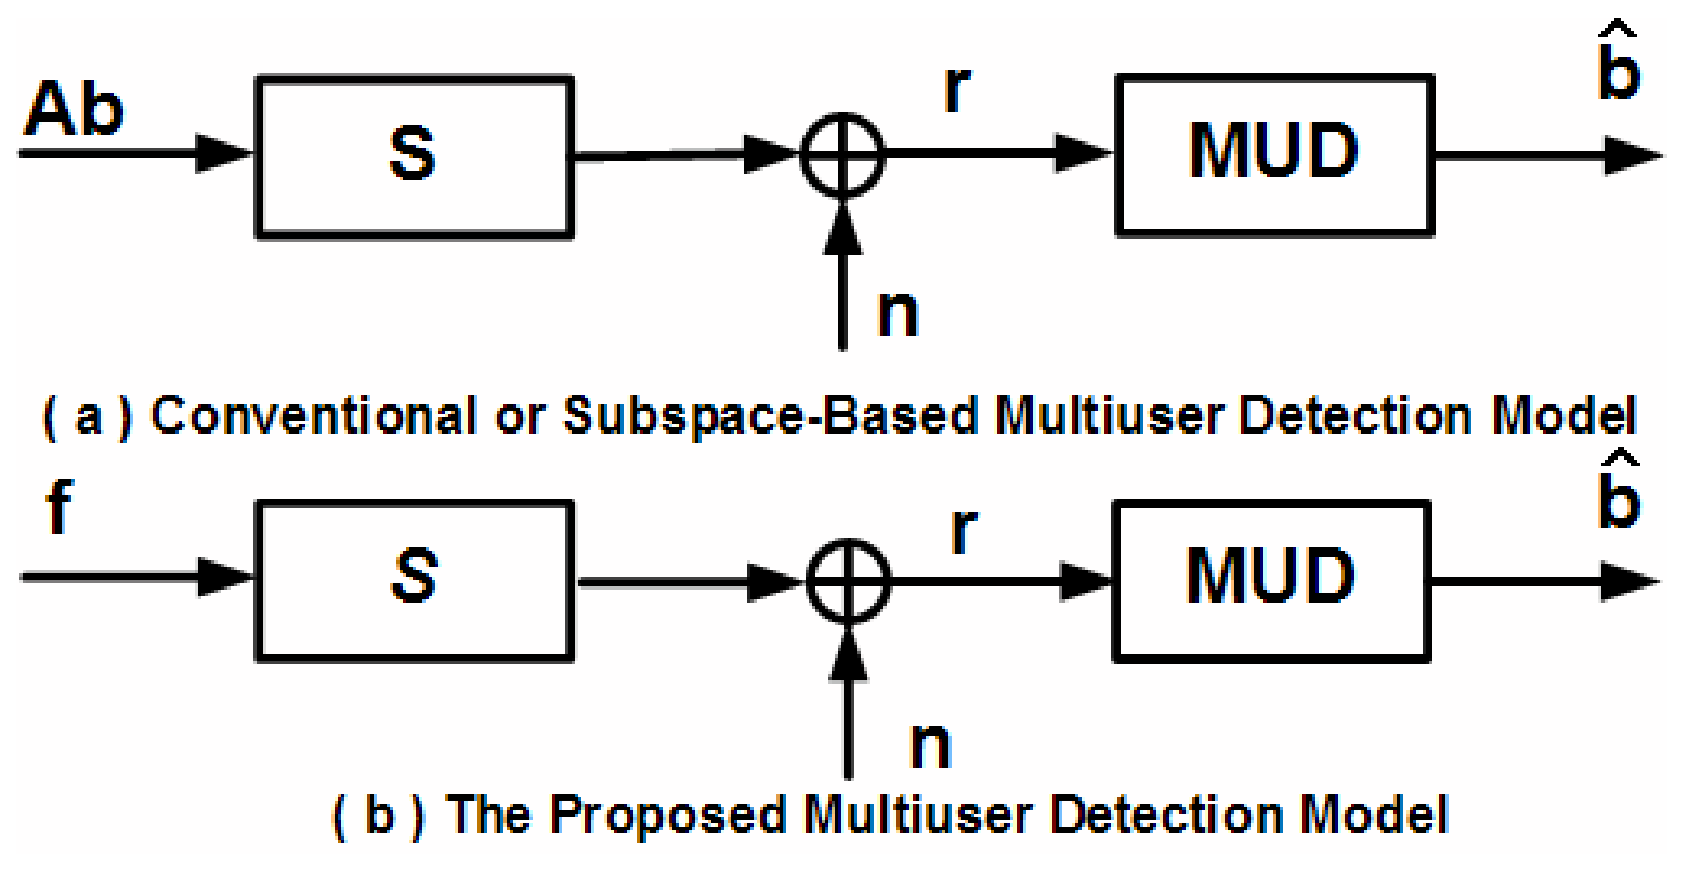
\includegraphics[width=2.5in]{MUD_model.eps}
\caption{Multiuser detection models.  } }\label{MUD_model}
\end{figure}
Instead of using the conventional signal model or the parametric
subspace signal model, we develop a new blind multiuser signal
model shown in Fig. 1, which uses a blind but "faked" spreading
matrix $\bcS$ for desired user(s). We call $\bcS$ the blind but
"faked" spreading matrix because 1) it is composed by only desired
users' spreading sequences and previously received signals and 2)
it isn't the original one but works like the original one. With
the construction of $\bcS$, we can construct group-wise or single
blind detectors in the following. Without loss of the generality,
only the bits sent for first $G$ users are considered here and the
$L\times M$ blind spreading sequence matrix $\bcS$ is defined by
\begin{equation}
\begin{array}{rcl}
\bcS&=&[\matrix{\bs_1&\ldots&\bs_G&{\br}_{1}&{\br}_{2}&\ldots&{\br}_{M-G}}]\\
\end{array} \label{S_0}
\end{equation}
\noindent where $\bs_g$, $g=1,\ 2,\ \ldots,\ G$, denote the group
of $G$ spreading waveforms which are already known to user $1$.
${\br}_m$, $m=1,\ 2,\ \ldots,\ M-G$, are $M-G$ previously received
independent signal vectors~\footnote{The first $M-G$ received
signal $\br_m$ may be obtained from some receiver initialization
procedure. After that, there will be some possible adaptive
procedure for updating $\bcS$, e.g. the procedure proposed in
Section \ref{updatingG}. Compared with existing blind detectors,
this number, $M-G$, of required previously received signals are
very small.}. $K\leq M\leq L$, where $M=K$ is the minimum number
for blind multiuser detector to unambiguously distinguish
different interfering signals and $M\leq L$ is the constraint for
guaranteing the uniqueness of designed blind multiuser receiver.
The relationship between the proposed blind spreading matrix
$\bcS$ and the original spreading matrix $\bS$ can be given by
\begin{equation}
\begin{array}{rcl}
\bcS &=&\bS\bB + {\bN}\\
\end{array}\label{S_1}
\end{equation}
\noindent where the first $G$ columns of $\bcS$ and $\bS$ are
same,
\begin{equation}\hspace{-0.0in}
\begin{array}{c}
 \bB=\left[\matrix{\bI & \bar\bD\cr\bzero&\tilde\bD }\right]=\left[\matrix{\bE & \matrix{\bar\bD\cr \tilde{\bD}} }\right]
  =\left[\matrix{\bG \cr \matrix{\mathbf{0}& \tilde{\bD}}
 }\right]
\end{array}\label{B}
\end{equation}
\noindent is the $K\times M$ data matrix associated with $\bcS$.
$\bE=[\matrix{\bI&\bzero}]^{\rm T}$ is a $K\times G$ matrix, $\bG
= \left[\matrix{\bI& \bar\bD}\right]$ is the $G\times M$ matrix,
where $\bar\bD$ is previously detected and known matrix for
desired users. $\mbox{rank}\{\tilde{\bD}\}=K-G$, where
$\tilde{\bD}$ is unknown matrix for unknown $K-G$ users, and
$\mbox{rank}\{\bB\}\leq K$. Combining (\ref{r_sync}) and
(\ref{S_1}), the received signal vector $\br$ in (\ref{r_sync})
can be expressed as the linear combination of the columns in
$\bcS$ instead of $\bS$, which is written by
\begin{equation}
\begin{array}{rcl}
\br&=&\bcS\bbf + \bar{\bn} \label{r_blind}
\end{array}
\end{equation}
\noindent where the $M \times 1$ vector $\bbf$ is termed the
detection vector defined by
\begin{equation}
\begin{array}{rcl}
\bbf&=&\bB^{+}\bar\bb
\end{array} \label{DetectorVector}
\end{equation}
\noindent where $[\cdot]^{+} $ denotes the general inverse
operator and $\bar\bb=\bA \bb$. $\bar{\bn}$ is the new $L\times 1$
AWGN vector defined by
\begin{equation}
\begin{array}{rcl}
\bar{\bn}&=&\bn-{\bN}\bB^{+}\bar\bb
\end{array} \label{new_noise}
\end{equation}
We can see that (\ref{r_blind}) may be taken as a modified linear
prediction model and the multiuser detection problem may be taken
a modified linear prediction problem if $\bar{\bn}=\bzero$. On the
other hand, if $\bbf$ can be estimated, the amplitudes $A_g$ and
bits $b_g$ for the first $G$ users can be estimated and detected
with (\ref{DetectorVector}) by
\begin{equation}\hspace{0.2in}
\begin{array}{l}
\hat{\bb}_1
=\left[\matrix{\hat{b}_1&\hat{b}_2&\ldots&\hat{b}_G}\right]^{\rm
T}=\mbox{sgn}\left\{\bG\bbf\right\}\
\end{array}, \label{b_estimation}
\end{equation}
\begin{equation}\hspace{-0.40in}
\begin{array}{l}
\hat{\ba}_1
=\left[\matrix{\hat{A}_1&\hat{A}_2&\ldots&\hat{A}_G}\right]^{\rm
T}=\left|\bG\bbf\right|\ .
\end{array} \label{A_estimation}
\end{equation}
In the following, we will present various schemes for estimating
$\bbf$ and detecting $\bb_1$. An adaptive implementation will be
presented in Section \ref{updatingG}.
\section{Blind Multiuser Detectors\label{LBD}}
\subsection{Least Squares Detection } At first, we assume that
the measurements of $\bcS$ are assumed to be free of error. All
errors are confined to the received vector $\br$. Hence, the
detection vector can be estimated with solving the following
equation~\cite{Huff91,Golu96}
\begin{equation}
\begin{array}{rcccl}
{\bbf}_{\rm
LS}&=&\matrix{\mbox{arg}\min\limits_{\bx}\left\|\br-\bcS\bx\right\|_2}&=&\bcS^+\br
\end{array}
\label{LSProb}
\end{equation}
\noindent and the bit vector for the first $G$ users can be
detected by
\begin{equation}
\begin{array}{rcl}
\hat{\bb}_1&=&\mbox{sign}\left\{\bG\bcS^{+}\br\right\}
\end{array} \label{b_LS}
\end{equation}
\subsection{Total Least Squares Detection}
The previous LS estimation assumes $\bcS$ to be error-free. This
assumption is not entirely accurate with $\bcS$ because of $\bN$.
Problem (\ref{LSProb}) can then be transformed into the TLS
problem:
\begin{equation}
\begin{array}{l}
\left[\matrix{\bcS_{\rm TLS}\cr\bbf_{\rm
TLS}}\right]=\matrix{\mbox{arg}\min\limits_{\bar{\bcS},\
\bx}\left\|\left[ \matrix{\bcS\cr\br} \right] - \left[
\matrix{\bar{\bcS}\cr\bar{\bcS}\bx}\right]\right\|_2}
\end{array}.
\label{TLSProb}
\end{equation}
 Let $\bcS=\bU^{'}\mathbf{\Sigma}^{'}\bV^{'\rm T}$ and
$[\bcS\ \br]=\bU\mathbf{\Sigma}\bV^{\rm T}$ be the SVD of $\bcS$
and $[\bcS\ \br]$, respectively. If $\sigma_K^{'}
> \sigma_{K+1}$, TLS estimation of $\bbf$ then is~\cite{Huff91,Golu96}
\begin{equation}
\bbf_{\rm TLS} = \left(\bcS^{\rm
T}\bcS-\sigma_{K+1}^2\bI\right)^{-1}\bcS^{\rm T}\br
\end{equation}
\noindent and the bit vector for the first $G$ users can be
detected by
\begin{equation}
\begin{array}{rcl}
\hat{\bb}_1&=&\mbox{sign}\left\{\bG(\bcS^{\rm
T}\bcS-\sigma_{K+1}^2\bI)^{-1}\bcS^{\rm T}\br\right\}
\end{array} \label{b_TLS}
\end{equation}
\subsection{Mixed LS/TLS Detection}
Though there exists a noise or error matrix $\bN$ in $\bcS$, its
first $G$ columns are exactly known to be noise-free or
error-free. Hence, to maximize the estimation accuracy of the
detection vector $\bbf$, it is natural to require the
corresponding columns of $\bcS$ to be unperturbed since they are
known exactly. Problem (\ref{LSProb}) and (\ref{TLSProb}) can then
be transformed into the following MLS problem:
\begin{equation}
\begin{array}{l}
\left[\matrix{\bcS_{\rm MLS}\cr\bbf_{\rm
MLS}}\right]=\matrix{\mbox{arg}\min\limits_{\bar{\bcS},\
\bx}\left\|\left[\matrix{\tilde{\bcS}\cr\br}\right]-\left[\matrix{\bar{\bcS}\cr[\bs_1\
 \bar{\bcS}]\bx}\right]\right\|_{2} }
\end{array}.\label{MLSProb}
\end{equation}
Perform the Householder transformation $\bQ$ on the matrix
$[\matrix{\bcS&\br}]$ so that
\begin{equation}\hspace{-0.14in}
\begin{array}{l}
\bQ^{\rm
T}[\matrix{\bs_1&\ldots&\bs_G&\bar{\bcS}&\br}]=\left[\matrix{\bR_{11}&\bR_{12}&\br_{1r}\cr
\mathbf{0}&\bR_{22}&\br_{2r}}\right]
\end{array}
\end{equation}
where $\bR_{11}$ is a $G\times G$ upper triangle matrix,
$\br_{1r}$ is a $G\times 1$ vector and $\br_{2r}$ is a
$(L-G)\times 1$ vector. Denote $\sigma'$ as the smallest singular
value of $\bR_{22}$ and $\sigma$ as the smallest singular value of
$[\matrix{\bR_{22}&\br_{2r}}]$. If $\sigma'>\sigma$, then the MLS
solution uniquely exists and is given by~\cite{Huff91}
\begin{equation}\hspace{-0.09in}
\begin{array}{rcl}
\bbf_{\rm MLS}&=&\left(\bcS^{\rm
T}\bcS-\sigma^2\left[\matrix{\bzero&\mathbf{0}\cr\mathbf{0}&\mathbf{I}_{M-G}}\right]\right)^{-1}\bcS^{\rm
T}\br
\end{array}.
\end{equation}
\noindent and the bit vector for the first $G$ users can be
detected by
\begin{equation}\hspace{-0.2in}
\begin{array}{l}
\hat{\bb}_1=\mbox{sign}\left\{\bG\left(\bcS^{\rm
T}\bcS-\sigma^2\left[\matrix{\bzero&\mathbf{0}\cr\mathbf{0}&\mathbf{I}_{M-G}}\right]\right)^{-1}\bcS^{\rm
T}\br\right\}
\end{array} \label{b_MLS}
\end{equation}
\subsection{Best Linear Unbiased Detection}
We assume the linear structure
\begin{equation}
\begin{array}{rcl}
{\bbf}_{\rm BLU}&=&\bW_{\rm BLU}^{\rm T}\br
\end{array}
\end{equation}
\noindent for this so-called best linear unbiased estimator
(BLUE), which is equal to the optimal minimum variance unbiased
estimator (MVUE) in linear signal models if the data are truly
Gaussian. Matrix $\bW_{\rm BLU}$ is designed such that: 1) $\bcS$
must be deterministic, 2) $\bar{\bn}$ must be zero mean with
positive definite known covariance matrix $\bC_{\bar{\bn}}$, 3)
${\bbf}_{\rm BLU}$ is an unbiased estimator of $\bbf$, 4) and the
error variance for each of the $M$ parameters is minimized as
\begin{equation}
\begin{array}{rcl}
\bW_{\rm BLU}&=&\min\limits_{\bW_{\bbf}}
\mbox{var}\left\{\bW_{\bbf}^{\rm T}\br\right\}
\end{array}.
\end{equation}
\noindent The resulting best linear unbiased estimator is
(Gauss-Markov Theorem):
\begin{equation}
\begin{array}{rcl}
{\bbf}_{\rm BLU}&=&(\bcS^{\rm
T}\bC_{\bar{\bn}}^{-1}\bcS)^{-1}\bcS^{\rm
T}\bC_{\bar{\bn}}^{-1}\br\ .
\end{array} \label{BLUE}
\end{equation}
\noindent The covariance matrix of ${\bbf}_{\rm BLU}$ given by
\begin{equation}
\begin{array}{rcl}
{\bC}_{\bbf_{\rm BLU}}&=&(\bcS^{\rm
T}\bC_{\bar{\bn}}^{-1}\bcS)^{-1}
\end{array}.
\end{equation}
\noindent Though the PDF of $\bB$ may be determined, the PDF of
$\bB^{+}$ is largely unknown. However, with Girko's Law, when
$\alpha=(K-G)/(M-G)$ is fixed, $K$, $M$ $\rightarrow\infty$, the
diagonal element of
$\frac{1}{M-G}\tilde{\bD}^+\tilde{\bb}\tilde{\bb}^{\rm
T}\tilde{\bD}^{\rm +T}$ may be approximated by~\cite{Muller}
\begin{equation}
\begin{array}{rcl}
\lim\frac{1}{M-G}\left[\tilde{\bD}^+\tilde{\bb}\tilde{\bb}^{\rm
T}\tilde{\bD}^{\rm +T}\right]_{ii}^{-1}&=&1-\alpha
\end{array}.
\end{equation}
\noindent Hence, the covariance matrix of $\bbf$, $\bC_{\bbf}$,
can be decided by
\begin{equation}
\begin{array}{rcl}
\bC_{\bbf}&=&\left[\matrix{\frac{2M-K-G}{M-K}\bA_1^2&\bzero^{\rm
T}\cr\bzero&\frac{1}{M-K}\bI}\right]
\end{array},
\end{equation}
\noindent where
$\bA_1=\mbox{diag}\left\{\left[\matrix{\hat{A}_1&\hat{A}_2&\ldots&\hat{A}_G}\right]\right\}$,
\begin{equation}
\begin{array}{rcl}
\bC_{\bar\bn}&=&\sigma^{2}\frac{2M-K-G}{M-K}\bI
\end{array}\label{noise_var_new}
\end{equation}
\noindent and the bit vector for the first $G$ users can be
detected by
\begin{equation}
\begin{array}{rcl}
\hat{\bb}_1&=&\mbox{sign}\left\{\bG(\bcS^{\rm
T}\bcS)^{-1}\bcS^{\rm T}\br\right\}
\end{array}
\end{equation}
\subsection{Minimum Mean Squared Error Detection}
Given measurements $\br$, the MMSE estimator of $\bbf$,
${\bbf}_{\rm MMSE} = f( \br )$, minimizes the MSE $J_{\rm
MSE}=E\{||\bbf-\hat{\bbf}||_2^2\}$. When $\bbf$ and $\br$ are
jointly Gaussian, the linear estimator $\bW_{\rm MMSE}$ that
minimizes the MSE $J_{\rm MSE}$ is (Bayesian Gauss-Markov
Theorem)~\cite{Haykin96}
\begin{equation}
\begin{array}{rcl}
{\bbf}_{\rm MMSE}&=&(\bC_{\bbf}^{-1}+\bcS^{\rm
T}\bC_{\bar{\bn}}^{-1}\bcS)^{-1}\bcS^{\rm
T}\bC_{\bar{\bn}}^{-1}\br\ ,
\end{array} \label{MSE}
\end{equation}
\noindent which is also termed Wiener filter, and the bit vector
for the first $G$ users can be detected by
\begin{equation}\hspace{-0.05in}
\begin{array}{l}
\hat{\bb}_1=\mbox{sign}\left\{\bG(\bC_{\bbf}^{-1}+\bcS^{\rm
T}\bC_{\bar{\bn}}^{-1}\bcS)^{-1}\bcS^{\rm
T}\bC_{\bar{\bn}}^{-1}\br\right\}
\end{array}
\end{equation}
\section{Adaptive Implementation\label{updatingG}}
\begin{figure}
\center{
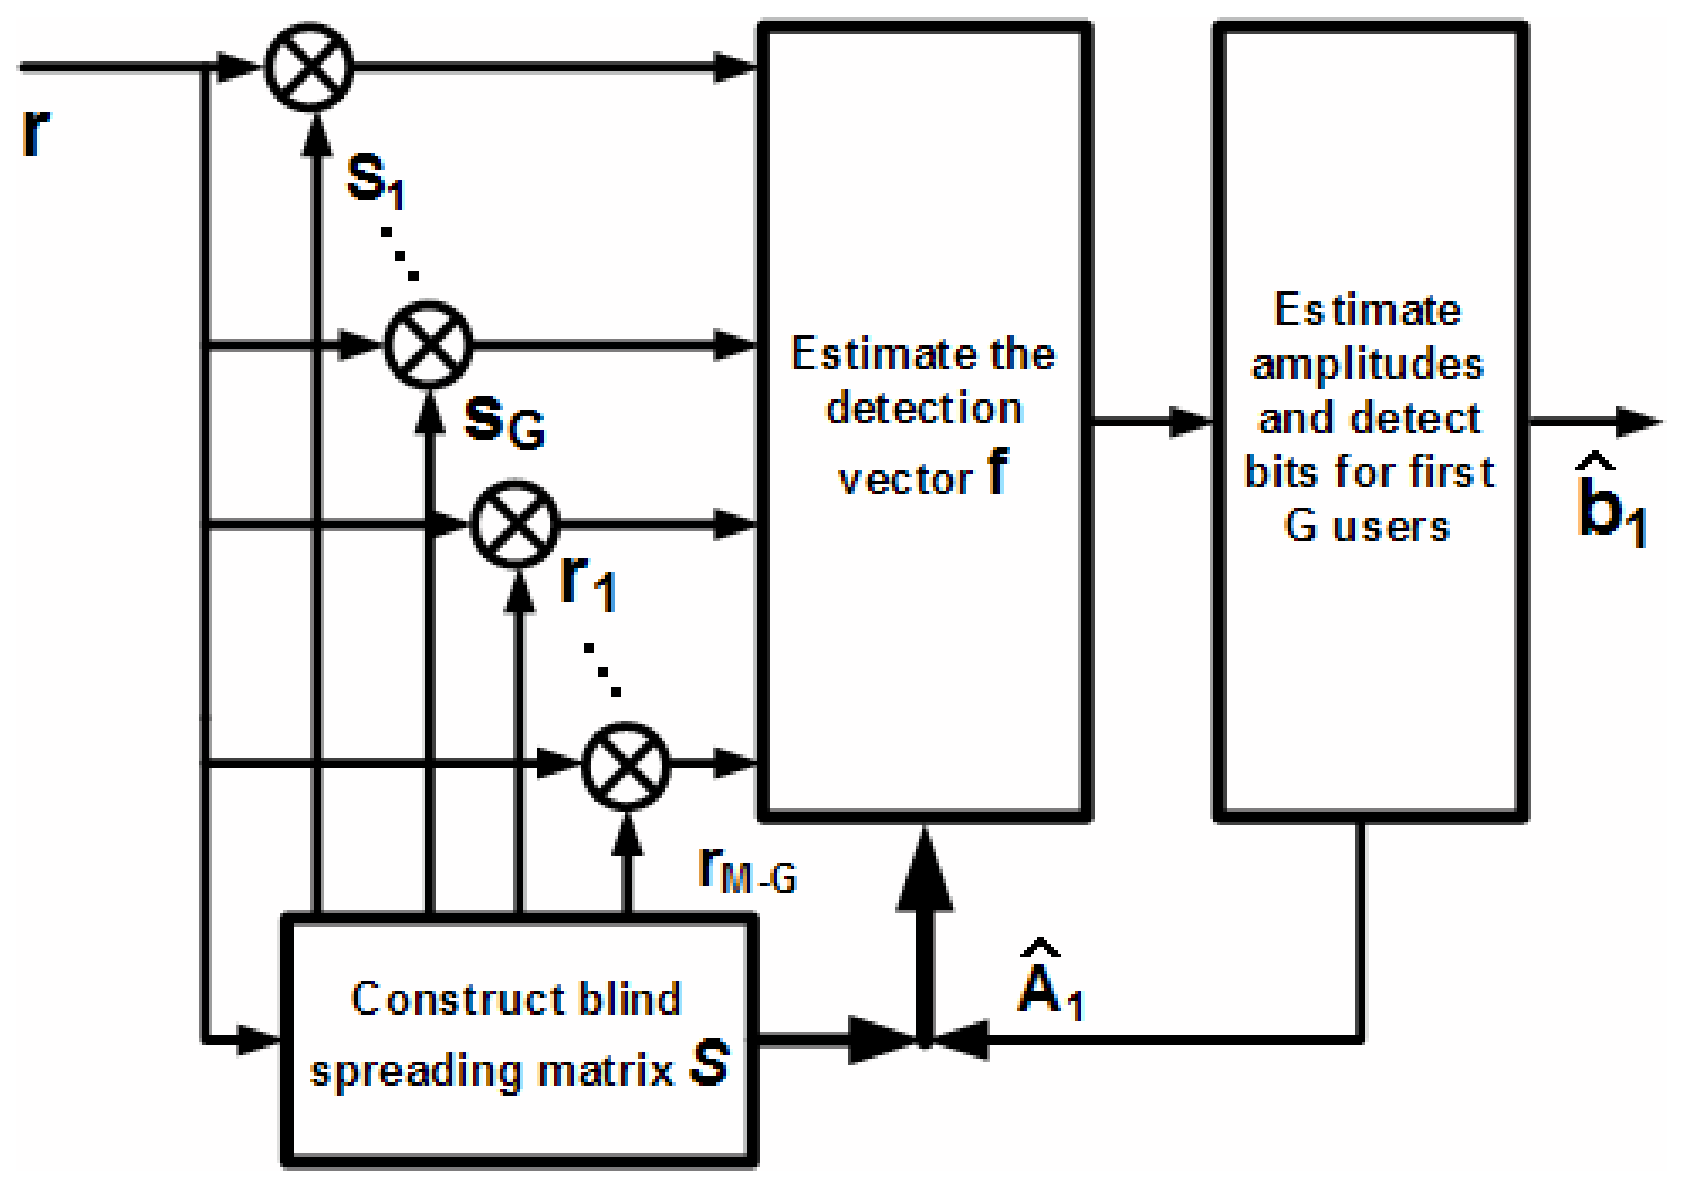
\includegraphics[width=2.5in]{BMUD_structure12.eps}
\caption{ The proposed adaptive blind multiuser detection
structure.} }\label{AMUDstruct}
\end{figure}
In Fig. 2, an adaptive structure of the presented blind multiuser
detection scheme is presented for time-variant channels. Following
the well-known Sherman-Morrison-Woodbury matrix inverse
lemma~\cite{Haykin96,Golu96}, a recursively adaptive
implementation of the proposed LS and BLU blind detector can be
expressed by
\begin{equation}\hspace{-0.0in}
\begin{array}{rcl}
\hat{\bb}_1(n)&=&\mbox{sign}\left\{\bG(n)\bcC_{\cal
S}^{+}(n)\bcS^{\rm T}(n)\br(n)\right\}
\end{array}
\end{equation}
\begin{equation}\hspace{-0.0in}
\begin{array}{l}
\bcC_{\cal S}^{+}(n)=\bcC_{\cal S}^{+}(n-1)-\frac{\bcC_{\cal
S}^{+}(n-1)\bu(n-1)\bu^{\rm T}(n-1)\bcC_{\cal
S}^{+}(n-1)}{1+\bu^{\rm T}(n-1)\bcC_{\cal S}^{+}(n-1)\bu(n-1)}
\end{array}\label{adaptiveLS}
\end{equation}
\noindent where
\begin{equation}\hspace{-0.0in}
\begin{array}{rcl}
\bcC_{\cal S}(n)&=&\bcS(n)^{\rm T}\bcS(n)
\end{array}
\end{equation}
 \noindent and $\bu(n-1)$ is designed using SVD so that
\begin{equation}\hspace{-0.00in}
\begin{array}{rcl}
\bu(n-1)\bu^{\rm T}(n-1)&=&\bcC_{\cal S}(n)-\bcC_{\cal S}(n-1)
\end{array}
\end{equation}
\section{Performance Analysis}
\subsection{AME and Near-Far Resistance}
A commonly used performance measure for a multiuser detector is
asymptotic multiuser efficiency (AME) and near-far
resistance~\cite{Verd98}. Since the proposed algorithms converge
to the conventional decorrelating detector as $\sigma^2\rightarrow
0$, their AME and near-far resistance are identical to the
decorrelating detector:
\begin{equation}
\begin{array}{rcl}
\bar{\eta}_k&=&\frac{1}{\bR_{kk}^{+}}
\end{array}.
\end{equation}
\subsection{CRLB for $\bbf$ Estimation}
The Cram\'{e}r-Rao Lower Bound (CRLB) is given by the inverse of
the Fisher information matrix (FIM). Providing the blind spreading
matrix $\bcS$ is known beforehand, we first define the parameter
vector $\mathbf{\phi} = \left[\bar{\sigma}^{2}\ \bbf^{\rm
T}\right]^{\rm T}$, where $\bar{\sigma}^{2}
=(1+\frac{M-G}{M-K})\sigma^{2}$, for computing the FIM
\begin{equation}
\begin{array}{rcl}
{\bI(\mathbf{\phi})} &=& {\rm E} \left\{ \left( \frac{\partial
\ln{\cal L}}{\partial \mathbf{\phi}} \right) \left( \frac{\partial
\ln{\cal L}}{\partial \mathbf{\phi}} \right)^{\rm H} \right\}
\label{fim}
\end{array}
\end{equation}
\noindent where $\ln{\cal L}$ is the log-likelihood function given
by
\begin{equation}
\begin{array}{rcl}
\ln{\cal
L}&=&C-L\ln\bar{\sigma}^2-\frac{1}{2\bar{\sigma}^2}\parallel\mathbf{e}\parallel_2^2
\end{array},\label{logl}
\end{equation}
\noindent $C$ is a constant and $\mathbf{e}=\br-\bcS\bbf$.
Providing $\bcS$ is known, the closed-form CRLB expression of
$\bbf$ is then given by
\begin{equation}
\begin{array}{rcl}
{\rm CRLB}(\bbf\ |\ \bcS) &
=&(1+\frac{M-G}{M-K})\sigma^{2}(\bcS^{\rm T}\bcS)^{\rm +}
\end{array}.\label{CRLB_f}
\end{equation}
\noindent It shows that the accuracy of estimating $\bbf$ may
increase with increasing $M$.
\section{Computer Simulations}
\begin{figure} \center{
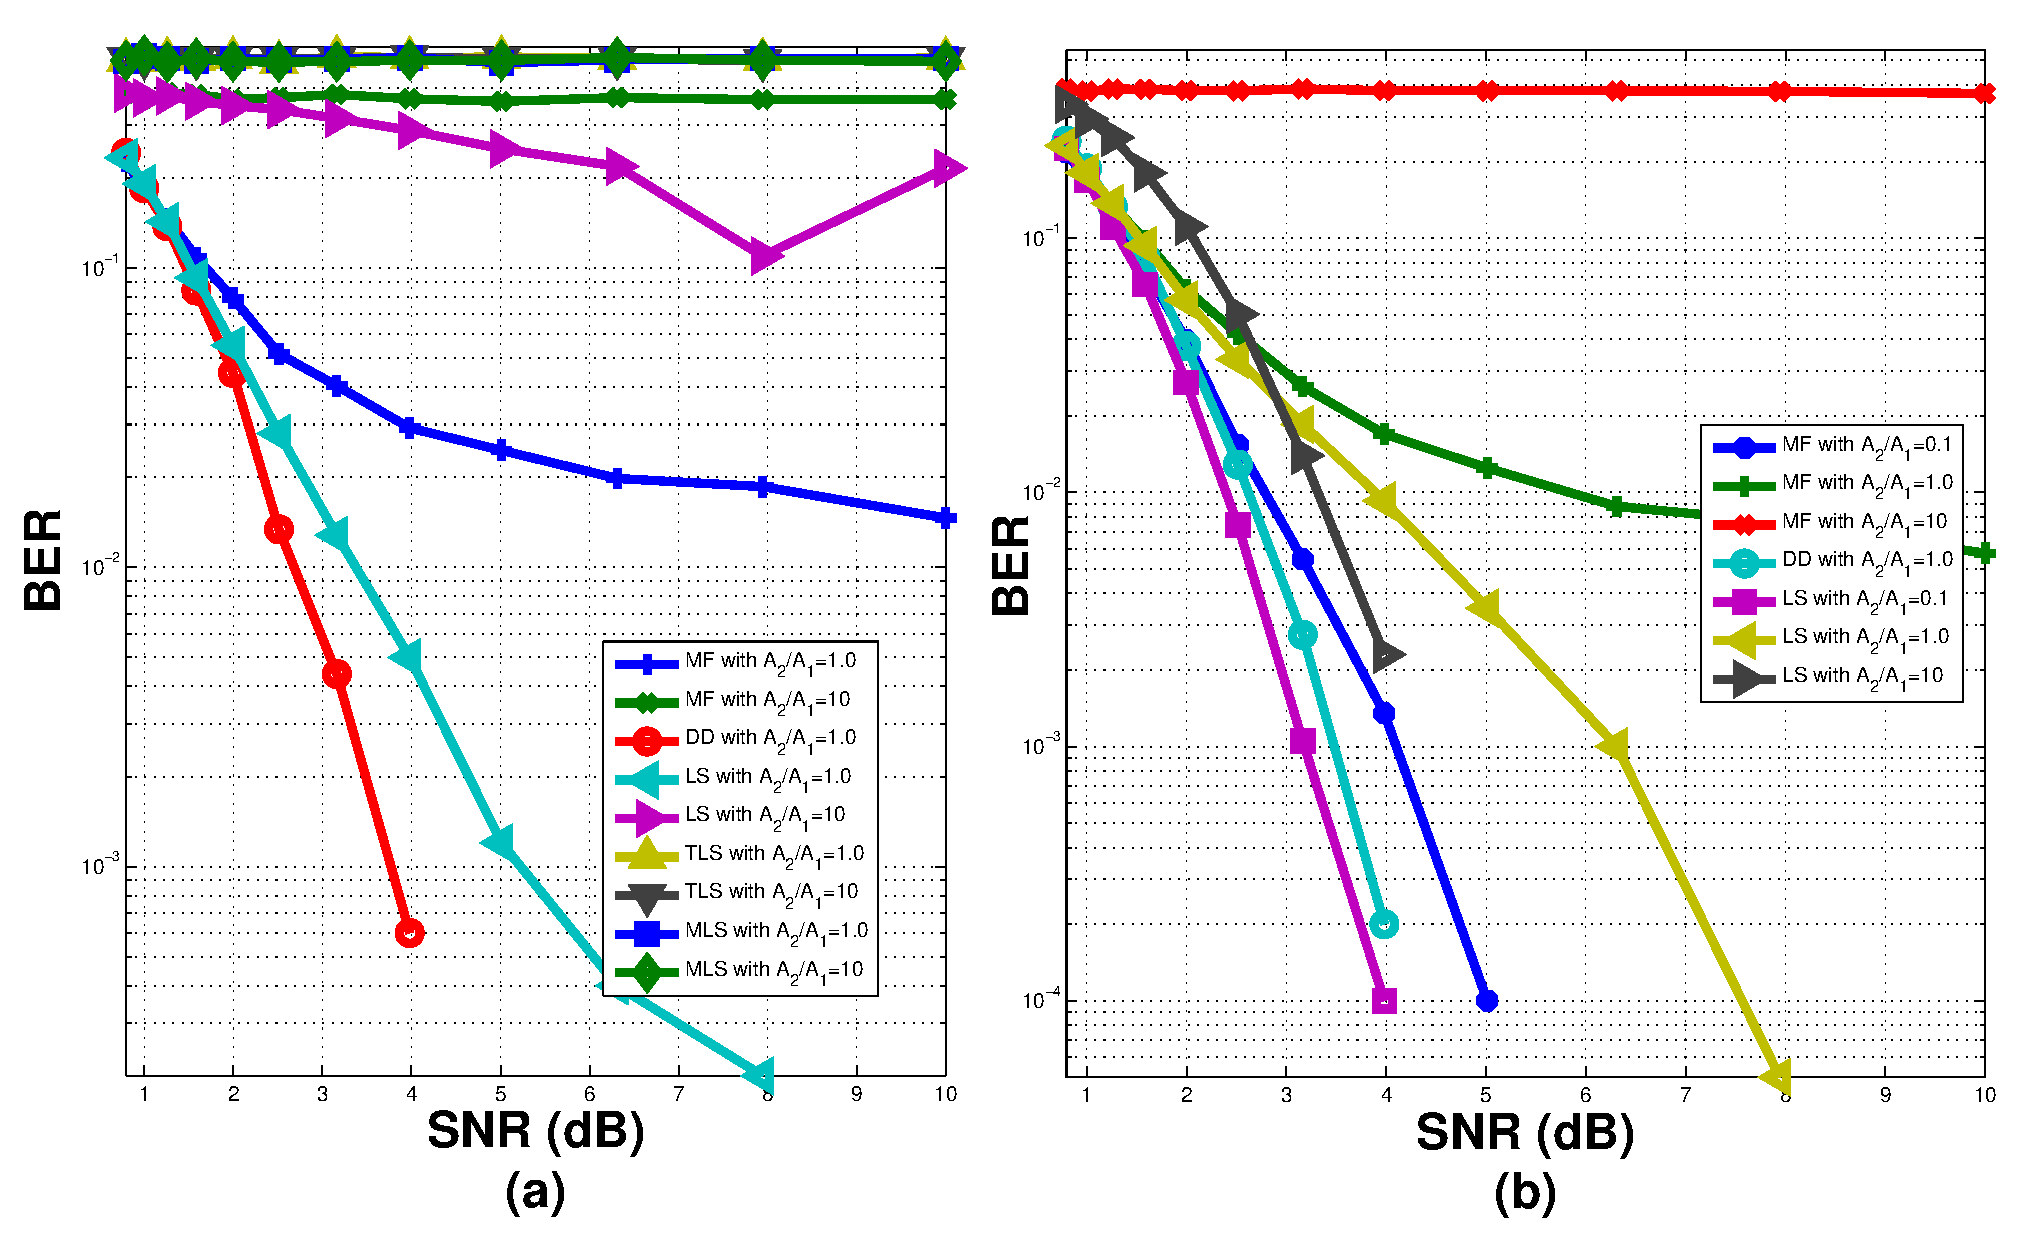
\includegraphics[width=2.5in]{BER_SNR_10_64.eps}
\caption{ (a) The performance of the proposed blind MUDs against
SNR, $M=12$. (b) The performance of the proposed blind LS
detector, $M=63$. } }\label{BER_SNR}
\end{figure}
\begin{figure} \center{
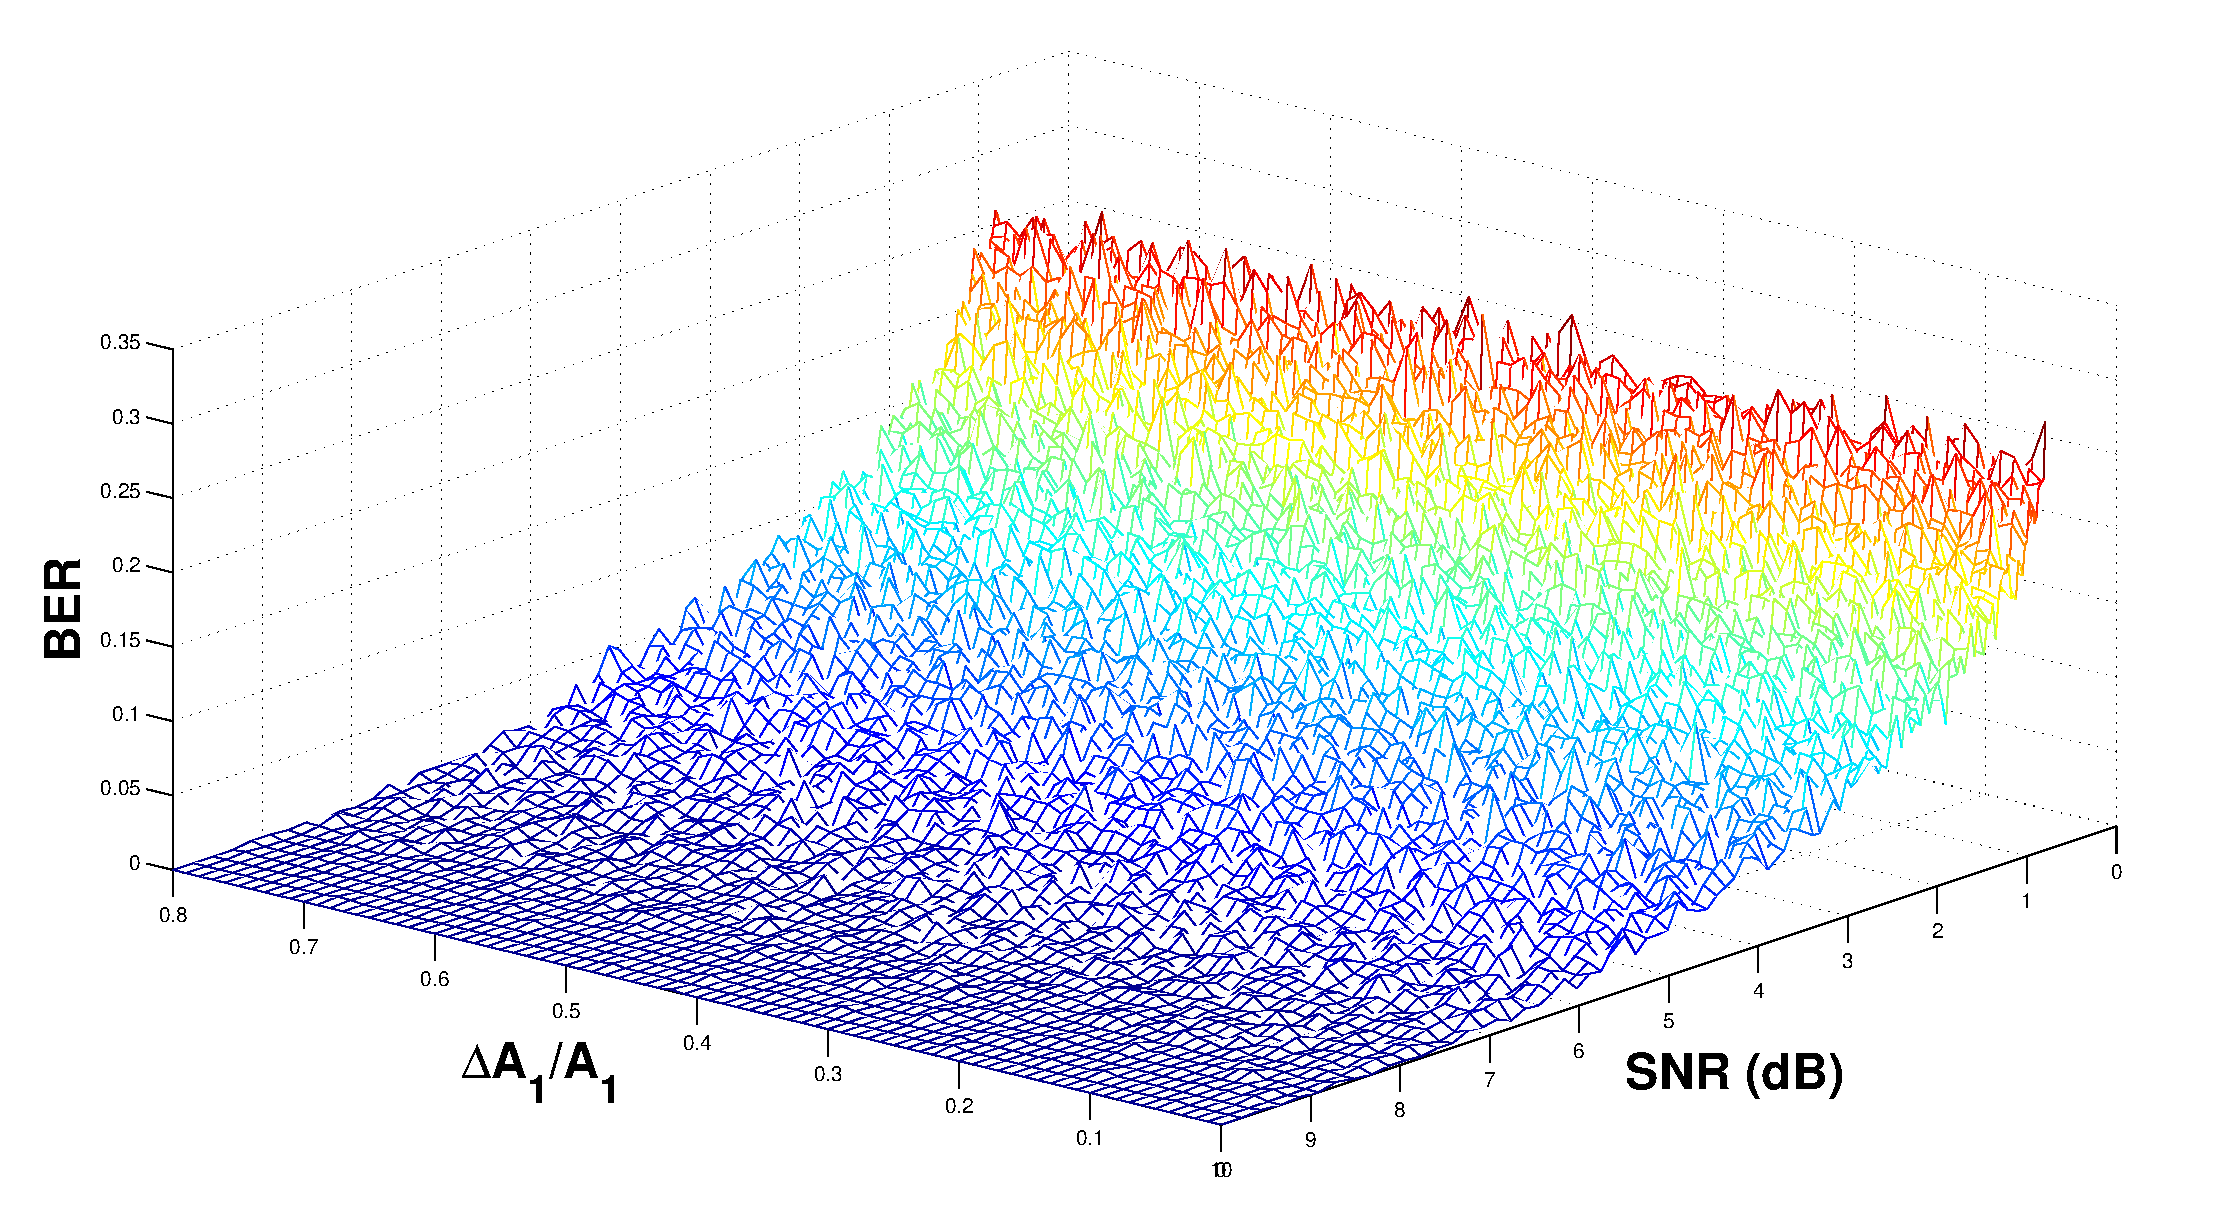
\includegraphics[width=2.5in]{BER_A_SNR_10_64_LSs.eps}
\caption{ The performance of the LS detector against amplitude
estimation error ${\Delta}{A_1}/A_1$ and SNR, $M=63$.}
}\label{BER_A_SNR}
\end{figure}
\begin{figure}
\center{
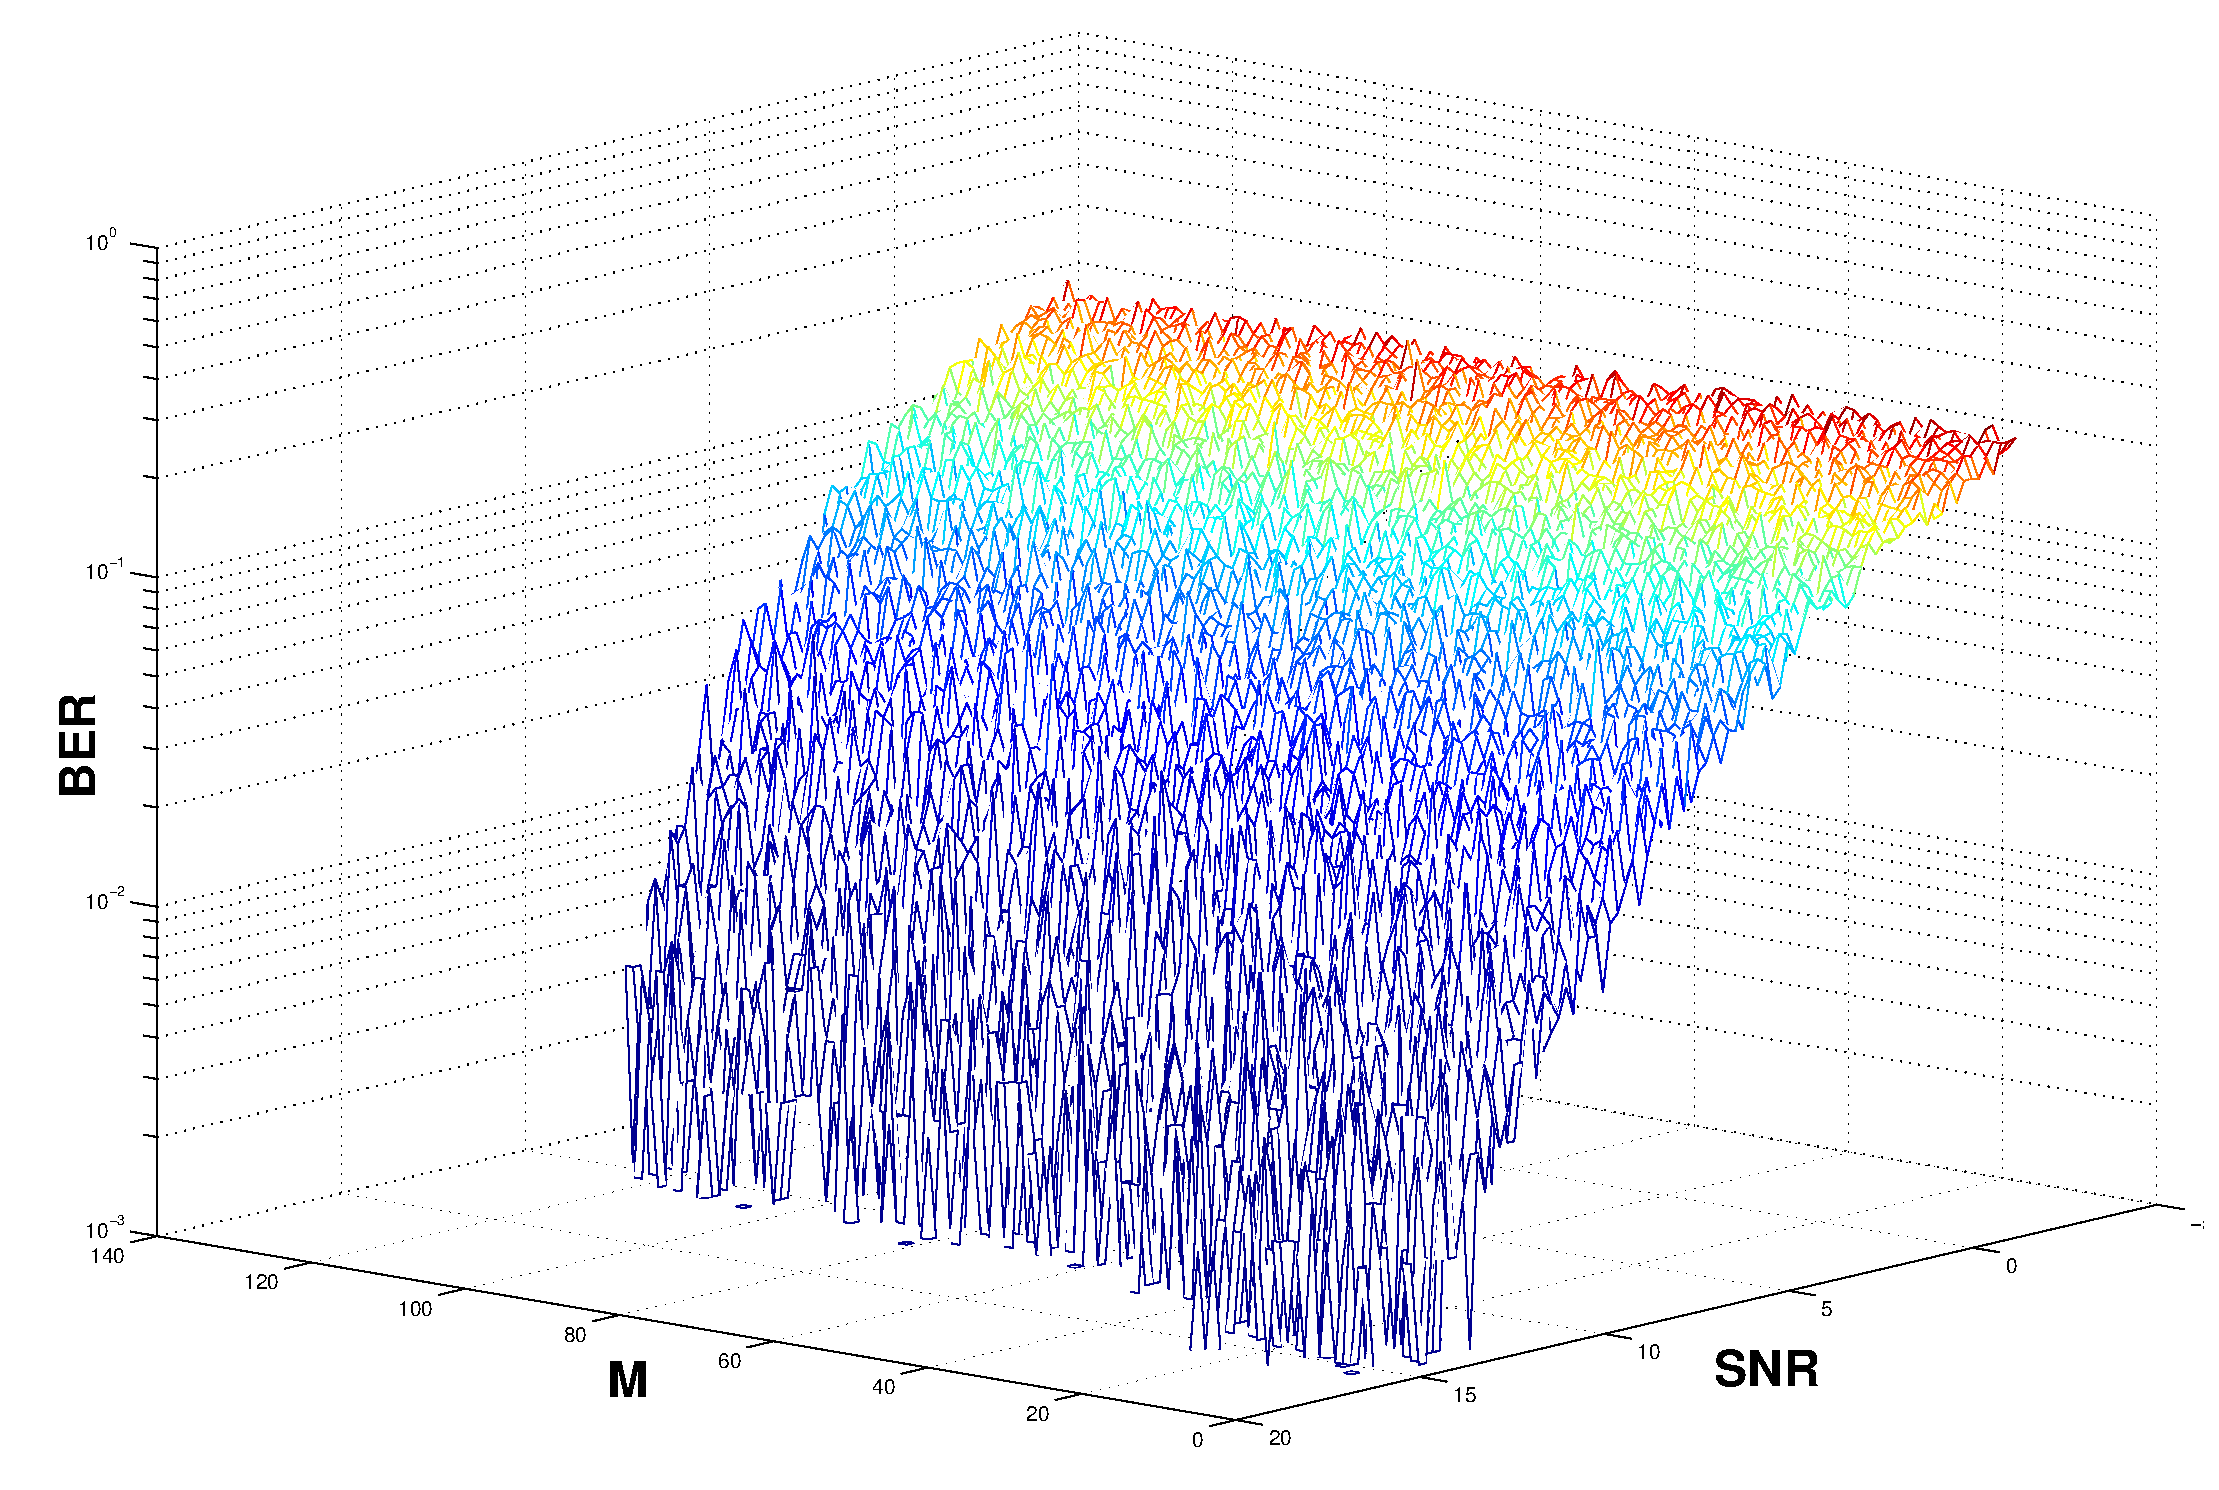
\includegraphics[width=2.5in]{BER_M_SNR_10_64_LSs.eps}
\caption{ The performance of the LS blind MUD against $M$ and
SNR.} }\label{BER_M_SNR}
\end{figure}
There are $K=10$ users with the group size $G=3$ and the spreading
sequences used in simulations are $64$-chip ($L=64$) random
sequences. In the computer simulations, the previous amplitude
estimation from (\ref{A_estimation}) is directly use for the next
detection without any amplitude filtering. From Subplot (a) in
Fig. 3, it is interesting to see that the performance of the
simplest LS detector has the best performance. From Subplot (b),
it is very impressive to find that the performance of blind LS
detector is very close to the conventional decorrelating detector
even with a strong MAI in our simulations when $M$ is large
enough. We then check the performance of the proposed LS blind
detector against the amplitude estimation errors. From Fig. 4, we
can see that the BER of the LS detector basically is unchanged
against amplitude estimation error when SNR is large enough. From
Fig. 5, we can see that the performance of the LS detector can be
better providing $M$ is larger enough. This confirms
(\ref{noise_var_new}), which shows that the variance of
$\bar{\bn}$ decreases with increasing $M$.
\section{Conclusions}
In this paper, we proposed a blind multiuser detection framework
as well as several blind detectors. The proposed blind detectors
are direct and simple without any channel or spreading sequence
estimation or subspace separation operation. The performance of
the proposed blind LS and BLU detectors are comparable with the
conventional decorrelating detector.

\small
\bibliographystyle{unsrt}
\bibliography{FastBDD}
\end{document}
